\subsection{Задача відновлення ваг для ланцюга}
Для зваженого графа ${\bf A_n} = (A_n,w)$, який є ланцюгом, розглянемо поставлену задачу.

Пронумеруємо його вершини від $1$ до $n$, тобто $ V({A_n}) = \{ 1,2,...,n\} $, і вершина $k$ суміжна з вершинами $k-1$ і $k+1:\ \forall k \in \{2,...,n-1\}$. Вагу ребра, що з'єднує $i$ та $i+1$ вершини $\forall i \in \{1,...,n-1\}$, позначимо $a_i$. 
\begin{figure}[H]
    \centering
    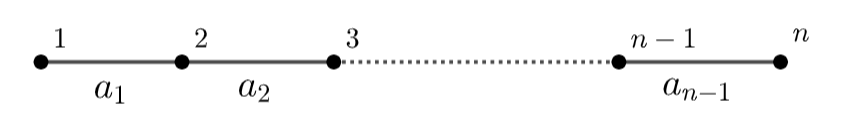
\includegraphics[width=0.9\linewidth]{pictures/An.png}
    \caption{$\bf A_n$}
    \label{An:image}
\end{figure}
Розглянемо випадок, коли $n = 2$.\\
Для ${\bf A_2}:\ \sigma({\bf A_2}) = \{-a_1,a_1\}$ і $P_{\bf A_2} = \lambda^2
- a_1^2$. Очевидно, що з такого спектра однозначно відновлюються ваги. Оскільки $a_1^2 = b$, де $b$ --- коефіцієнт многочлена, який відомий нам за умовою, то $a_1 = \sqrt{b},\ a_1>0$.

\textbf{Твердження 1.\label{Tv1}}\\
Для будь-якого $n\geq3$ можна відновити зважений граф $\bf A_n$ за спектром всього графа $\sigma({\bf A_n})$ і підспектром $\sigma({\bf A_{n-1}})$.